%!TEX root = ../terrainbook.tex
% chktex-file 46

\setchapterpreamble[u]{\margintoc}
\graphicspath{{gdem/figs/}}


\chapter{Global digital elevation models}% or global terrains
\label{chap:gdem}

We define as ``global digital elevation models'' (or global terrains) the datasets that cover (most of) the Earth (gDEM below).%
\index{global DEM}
Those datasets require different acquisition methods from the local ones, since flying an airplane or performing local surveys at the scale of the Earth is not really feasible (or is it?).
The acquisition instruments used must be space-borne, \ie\ mounted on a satellite for instance.

gDEMs are useful in several applications, especially for environmental studies such as geological studies, hydrological modelling, ecosystems dynamics.

gDEMS have several properties and characteristics that apply only to them, and we report in this chapter on the main ones.
% We first describe global acquisition techniques, then we discuss the properties (and errors and biases, etc.) that the datasets collected will have, 


Overview of apps:
@article{Yang11,
  author = {Liping Yang and Xingmin Meng and Xiaoqiang Zhang},
  journal = {International Journal of Remote Sensing},
  number = {14},
  pages = {3875--3896},
  title = {{SRTM} {DEM} and its application advances},
  volume = {32},
  year = {2011}}



%%%%%%%%%%%%%%%%%%%%
%
\section[Acquisition of global data]{Acquisition of global elevation data}

The acquisition of gDEMs requires the use of a sensor mounted on a satellite.

The first gDEM (SRTM v1) was constructed with InSAR and released in 2003. 

As an alternative to InSAR and images from satellite is lidar.



%%%
\subsection{InSAR}


%%%
\subsection{Photogrammetry from high-resolution satellite images}


%%%
\subsection{Space lidar (ICESat-2 + GEDI)}

Lidar was first used in space on the Apollo missions, and with further technological developments, it has been used extensively from the 1990s onwards.
For example, Mercury, Mars, near-earth asteroids, and lately again the moon have been scanned using lidar.

Earth surface elevation lidar measurements have also been developed, often flown on the Space Shuttles.
ICESat was the first earth-based lidar satellite, launched in 2003, with the primary goal of ice sheet monitoring.
It had an elevation accuracy of several cm and was operational for five years.

NASA launched in 2018 two missions measure the elevation of the Earth globally with lidar instruments:
\begin{enumerate}
  \item \textbf{GEDI}\marginnote{\url{https://gedi.umd.edu/}} (Global Ecosystem Dynamics Investigation) is attached to the international space station (ISS) and its main goal is to investigate global ecosystems.
  GEDI has been combined with TanDEM-X data to produce biomass estimates and with Landsat imagery to produce a global canopy height map.
  \item \textbf{ICESat-2}\marginnote{\url{https://icesat-2.gsfc.nasa.gov/}} (Ice, Cloud, and Land Elevation Satellite-2) is in a polar orbit to investigate ice sheets using its \emph{Advanced Topographic Laser Altimeter System} (ATLAS). 
  Apart from terrain retrieval, ICESat-2 also measures the surface, such as canopy height, and has many other applications such as measuring bathymetry and estimating biomass.
\end{enumerate}
\begin{figure}
  \centering
  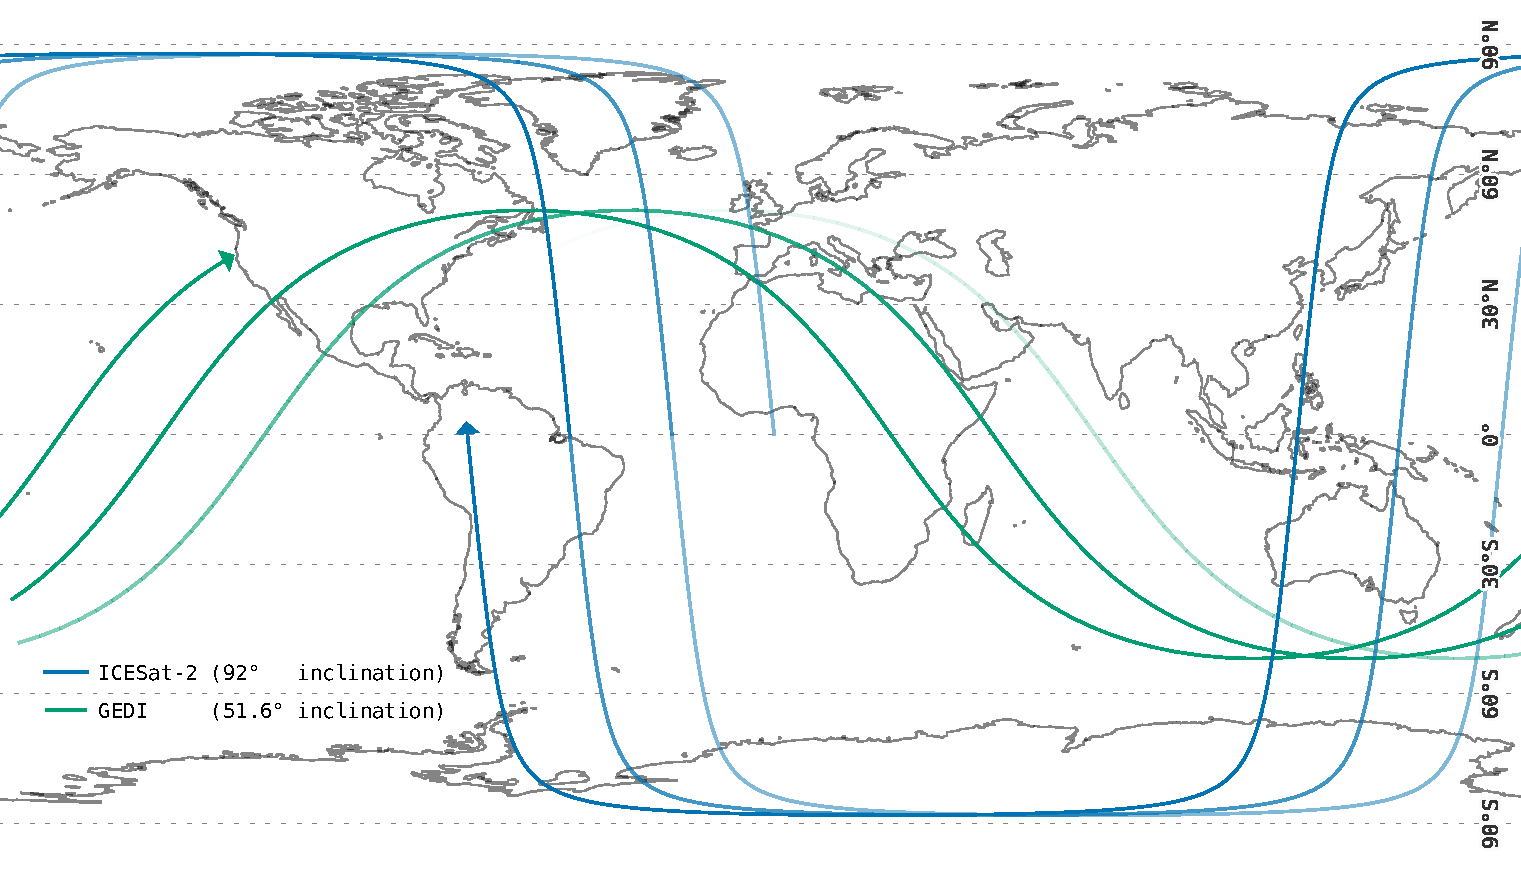
\includegraphics[width=\linewidth]{orbit}
  \caption{Three successive ground tracks for ICESat-2 and GEDI\@. Note the increased density of ground tracks at the latitude of inclination, as well as the lack of coverage beyond \ang{51.6}~latitude for GEDI.}%
\labfig{fig:orbit}
\end{figure}



The characteristics of both missions are summarised in Table~\ref{table:spacelidar}
\begin{table*}
  \sisetup{detect-weight=true,detect-inline-weight=math}
  \caption{Key characteristics of GEDI and ICESat-2 missions in comparison with a typical airborne mission.}
  \centering
  \begin{tabular}{llll}
    \toprule
    \ Mission              & ICESat-2                             & GEDI                                   & Typical airborne \\
    \midrule
    \ Type                 & Discrete photon                      & Full waveform                          & Either           \\
    \ Objective            & Cryosphere monitoring                & Ecosystems                             & -                \\
    \ Duration             & 2019-2022                            & 2019-2021                              & Single flight(s) \\
    \ Orbit Inclination    & \ang{92}                             & \ang{51.6}                             & NA               \\
    \ Laser pulse power    & \qty{175}{{\mu}J}/\qty{45}{{\mu}J}   & \qty{10000}{{\mu}J}/\qty{5000}{{\mu}J} & NA               \\
    \ Elevation            & \qty{\pm480}{km}                     & \qty{\pm420}{km}                       & \qty{0.5}{km}    \\
    \ Beam footprint       & \qty{17}{m}                          & \qty{23}{m}                            & \qty{0.05}{m}    \\
    \ Along track spacing  & \qty{0.7}{m}                         & \qty{70}{m}                            & \qty{0.1}{m}     \\
    \ Across track spacing & \qty{3}{km}/\qty{90}{m} between pair & \qty{0.6}{km}                          & \qty{0.1}{m}     \\
    \ Swath width          & \qty{6.6}{km}                        & \qty{4.2}{km}                          & \qty{1}{km}      \\
    \ Beam frequency       & \qty{512}{nm} (green)                & \qty{1064}{nm} (near-infrared)         & Either           \\
    \ \# beams             & 6 (in 3 pairs)                       & 8                                      & 1                \\
      \bottomrule
  \end{tabular}%
\label{table:spacelidar}
\end{table*}
Both missions have multiple laser beams and a division in beam energy, resulting in weak and strong beams.
Weak beams (or coverage beams) are a way to improve coverage while still maintaining the mission requirement(s) for a specific power level with the strong beams.
Coverage is further increased for both missions by the ability to angle the instruments away from their reference ground tracks, preventing repetitions of the same ground track.

%

The data from the ICESat-2 and GEDI missions is made publicly available in several data products, categorised in subsequent Level 1, 2, and 3 data products, each higher-level derived from a lower-level product.
Level 1 products contains the raw telemetry, whereas Level 2 products contain directly usable geolocated data to which several corrections---such as accounting for atmospheric effects---are applied.
Data for Level 3 are aggregated versions of Level 2 products, which are smaller in filesize and easier to process.
ICESat-2 differentiates between a Level 3A, which are aggregated Level 2 data products, and a Level 3B, which are gridded versions of the aggregated Level 3A data products.
GEDI's Level 3 data product are gridded versions of Level 2 data products, like ICESat-2's Level 3B.
GEDI also has Level 4 data products, which are model outputs---like carbon estimates---based on Level 2 data.


%%%%%%%%%%%%%%%%%%%%
%
\section[Specific characteristics]{Specific characteristics of gDEMs}

\begin{itemize}
  \item often near-global, depends on the orbits
  \item CRS, especially vertical datums
  \item resolution (often in degrees)
  \item DSM (more than DTM)
  \item size of datasets
  \item void filling: \url{https://en.wikipedia.org/wiki/Shuttle_Radar_Topography_Mission#Void-filled_SRTM_datasets}
  \item errors
  \item integration with sea-level datasets
  \item accuracy affected by slope (most image-based products)
\end{itemize}


%%%%%%%%%%%%%%%%%%%%
%
\section[Most common products]{Most common products available}

We list only the ones available as open-access?
For instance AW3D is also available as 5m-grid, but €€€.

% TODO: remake the inheritance fig
\begin{figure}
  \centering
  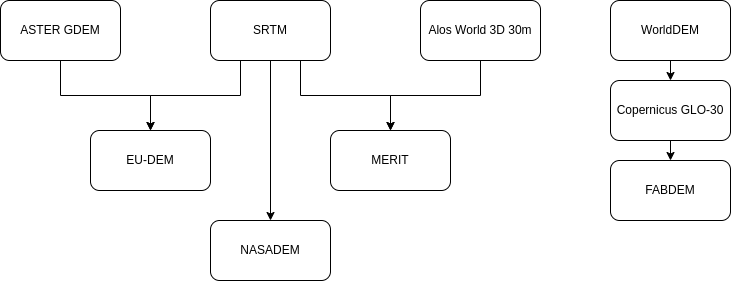
\includegraphics[width=\linewidth]{gdem_inheritance}
  \caption{(Figure from \url{https://github.com/DahnJ/Awesome-DEM})}%
\labfig{fig:gdem_inheritance}
\end{figure}

\begin{itemize}
  \item ASTER
  \item AW3D30
  \item STRM
  \item CopernicusDEM
  \item MERIT
  \item FABDEM
  \item ICESat-2 (the gridded version?)
  \item GEDI (the gridded version?)
  \item global proprietary (\url{https://github.com/DahnJ/Awesome-DEM#worlddem-and-tandem-x})
\end{itemize}

A few words about fusion? [Okolie22] has very long review.


%%%%%%%%%%%%%%%%%%%%
%
\section{Conversion DSM to DTM}

Some examples of how done?

Or: correction bias for vegetations/trees and buildings (all man-made objects).

%%%%%%%%%%%%%%%%%%%%
%
\section{Notes \& comments}


%%%%%%%%%%%%%%%%%%%%
%
\section{Exercises}

\begin{enumerate}
  \item What is what?
\end{enumerate}
